\begin{figure}[p]
 \caption{\footnotesize Separation plots for validation-period
    predictions of the ICEWS data (n=696).  For each model,
    observations are shown from left to right in order of increasing
    predicted probability of insurgency (shown as the black line).
    Observations where insurgency actually occurred are shown in
    red. EBMA outperforms all component models in assigning high
    predicted probabilities to \textit{more} observed insurgencies and
    to \textit{fewer} non-insurgencies.}
\label{InSam1sep}
\begin{center}
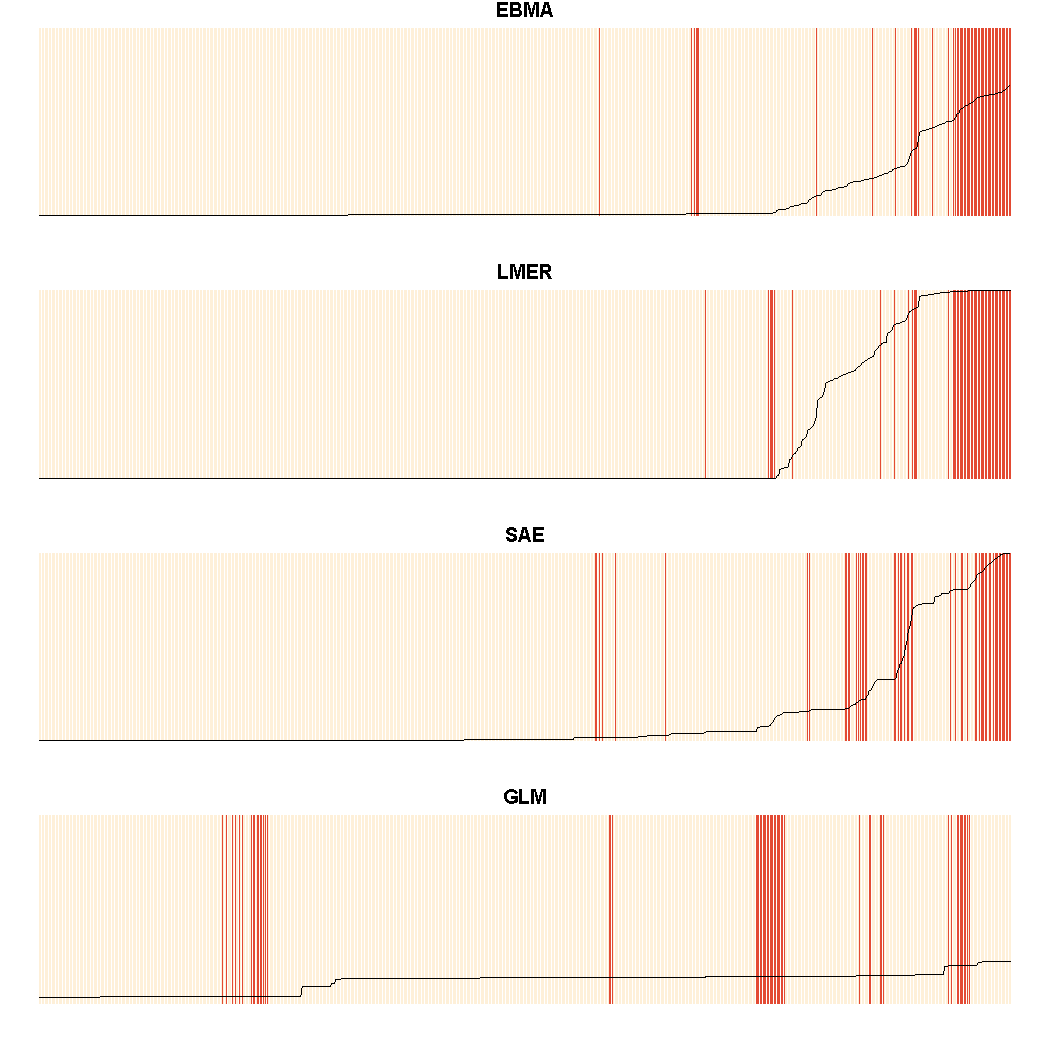
\includegraphics[width=4in]{Insample2-1.pdf}
\end{center}
\end{figure}

\begin{figure}
 \caption{\footnotesize Separation plots for the test-period
    predictions of the ICEWS data (n=348).  For each model,
    observations are shown from left to right in order of increasing
    predicted probability (shown as the black line).  Observations
    where insurgency actually occurred are shown in red.  EBMA
    outperforms all component models in assigning high predicted
    probabilities to \textit{more} observed insurgencies and to
    \textit{fewer} non-insurgencies.}
\label{OutSam1sep}
\begin{center}
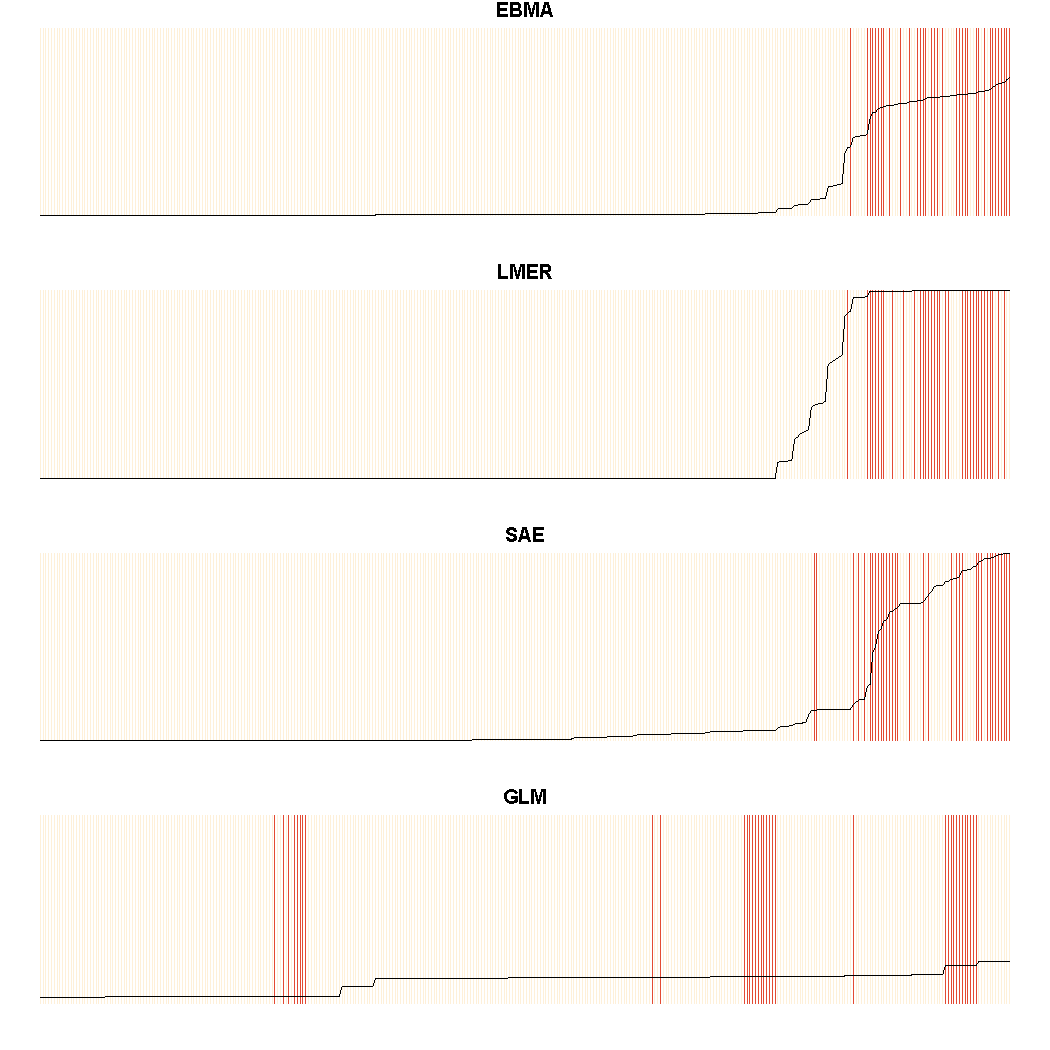
\includegraphics[width=4in]{OutSample2-1.pdf}
\end{center}
\end{figure}


 \begin{figure}[p]
   \caption{\footnotesize The predicted and actual percentage of the
     two-party vote going to the incumbent party in U.S. presidential
     elections from six component models and the EBMA forecast.  For
     each year, the plots show the point predictions (circles), 67\%
     predictive intervals (thick horizontal lines), and 90\%
     predictive intervals (thin horizontal lines).  The vertical
     dashed line is the observed outcome.  The EBMA model is
   better calibrated than its components. }
 \label{PresPlots2}
 \begin{center}
 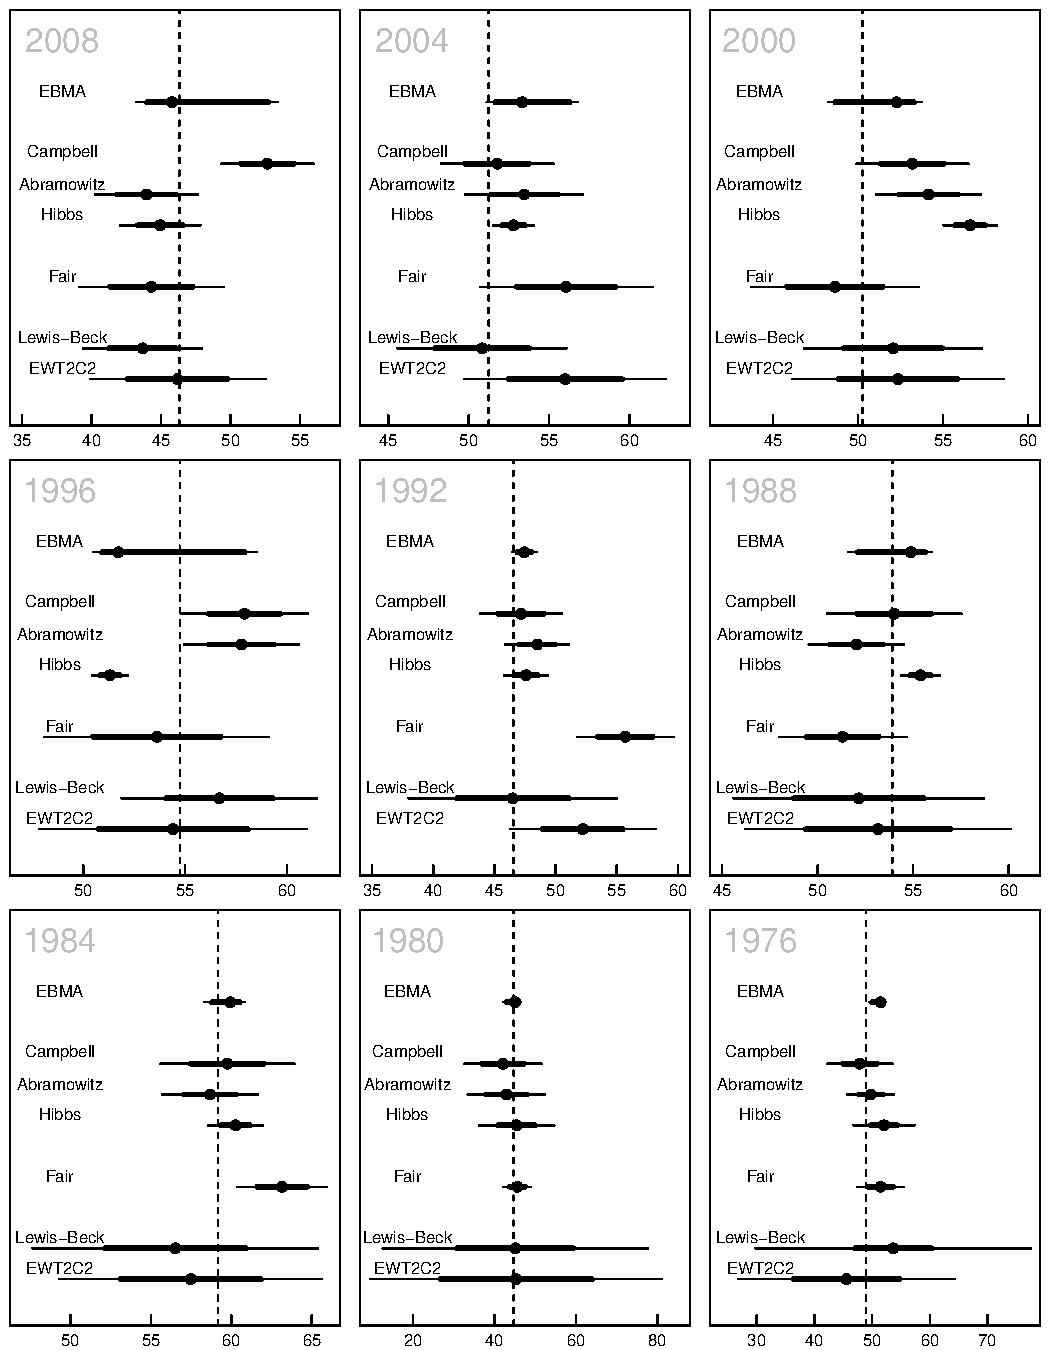
\includegraphics[width=5.6 in]{PresPlot2-1.pdf}
 \end{center}
 \end{figure}

